% Introduction

\pdfbookmark[1]{Quantitative revolutions}{Introduction}

\chapter{Quantitative revolution(s) in urban science}
\label{chap:quantitative_revolutions}

\begin{flushright}{\slshape    
And the first one now\\
Will later be last\\
For the times, they are a-changin'} \\ \medskip
--- Bob Dylan 
\end{flushright}


\bigskip


It is difficult to make a concise summary of what is known and not known about
urban systems. The vast amount of knowledge that has been gathered so far seems
very little in comparison to the bewildering complexity of the object being
studied~\cite{Batty:2008}. Every map, every satellite view, every statistic, every step
in cities elicits a question yet to be answered. What do we have to answer them?
A surprisingly small array of empirical tools and models. A surprisingly small
amount of solid, undisputed empirical facts.

Having said that, previous contributions are by no mean negligible. The body of
quantitative knowledge about cities has dramatically grown since the
quantitative revolution in Geography that took place after the $1950$s.
Recently, people have suggested that we may be witnessing the dawn of a second
quantitative revolution.\\

In the following Chapter, we will try to get some perspective on this claim, and
see to what extent it is justified. We will start with a (very) brief account of the
first quantitative revolution and the main themes around which it articulated
knowledge (a more comprehensive account can be found in~\cite{Sanders:2011}). We
will then critically review the factors traditionally invoked to justify the
spreading expression 'second quantitative revolution'.



\section{The first quantitative revolution}
\label{sec:the_first_quantitative_revolution}

Quantitative efforts in the study of human activities find their origin in Von
Th\"unen's model of agricultural land in $1826$, which suggests that the rent of land
should decay linearly with the distance to the city. More than a century later,
in $1933$, the German geographer Walter Christaller published his Central Place
Theory~\cite{Christaller:1933}, which aimed at explaining the size and location
of settlements in a system of cities. Needless to say, these early efforts are
theoretical in nature, and the empirical aspect -- studying things as they are
-- is left out. Surely due to the lack of available data.\\

The quantitative effort really starts to spread in the US in the
$1950$-$1960$~\cite{Berry:1993}. From the very beginning, the objective to make
geography a science is clearly stated. Starting with the introduction of Bunge's
seminal \emph{Theoretical Geography}, published in $1962$~\cite{Bunge:1962}.
According to the author, geographers can and should go beyond the mere
accumulation of facts, and try to discover the laws that rule the human and
physical phenomena occuring on the Earth's surface.   

Bunge proposed geometry as a tool to understand the observed pattern and
describe objectively the geographical space. The range of tools used quickly
expanded~\cite{Haggett:1966,Chorley:1968}, spanning stastistical
models~\cite{King:1969, Brunsdon:1998} -- whose importance is demonstrated by
the publication in $1969$ of Leslie King's \emph{Statistical Analysis in
geography}) -- and graph theory  -- as early as $1963$ with the publication of
Kansky's PhD thesis~\cite{Kansky:1963}. An early review of the use of graph
theory in geography can be found in Hagget and Chorley's
book~\cite{Haggett:1969}.\\

The research undertaken in the quantitative tradition can be -- tentatively --
divided in three different categories. First, the study of spatial
differentiation, aims at characterising the spatial patterns that result from
human activities. For instance, the study of population or employment densities
(see Part~\ref{part:polycentricity}), the local concentration of population
categories (see Part~\ref{part:segregation}), or the repartition of cities
inside a territory. 

Second, the study of spatial interactions. The progressive realisation that
distance is a critical factor to understand the arrangement of different spatial
phenomena led Tobler to state the First Law of Geography~\cite{Tobler:1970}. 

\begin{quote}
    Everything is related to everything else. But near things
    are more related than distant things.
\end{quote}

Linked to the study of spatial interactions is the (in)famous gravity model,
which states that the flow $F_{ij}$ between two locations $i$ and $j$ is given
by a function of the form

\begin{equation}
    F_{ij} = C\, P_i^\alpha\,P_j^\beta\, f(d_{ij})
\end{equation}

where $f$ is a decreasing function of distance. Although the analogy with
Newton's gravitation law was used by Reilly in $1931$ to find the retail market
boundaries between cities~\cite{Reilly:1931}, the above formulation in terms of
flows was formulated by Stewart in~\cite{Stewart:1948}. Note the competing
existence of Stouffer's theory of intervening
opportunities~\cite{Stouffer:1940}, according to which the flow between $i$ and
$j$ is proportional to the number of opportunities at $j$ and inversely
proportional to the number of opportunities between $i$ and $j$. It was
mathematically formulated later by Simini et al.~\cite{Simini:2012}.

Finally, the study of infrastructure. Starting with Kansky in
$1963$~\cite{Kansky:1963}, the study of the shape and growth of road networks,
railway networks and other infrastructure has witnessed a renewed interest
thanks to the study of spatial networks~\cite{Barthelemy:2011}.


\section{A second quantitative revolution?}
\label{sec:a_second_quantitative_revolution_}

People can be forgiven for believing that the present time bears any sort of
special character. But when we look closely enough, the change is perpetual, and
what is new now will be outdated tomorrow. During the past $3$ years, I have
at many times overheard the fact that we were currently witnessing a 'second
quantitative revolution' in the study of geographical systems. But is it really
the case? What differences with past tools or methods could justify such a
claim? In the following, we explore the three following hypotheses

\begin{itemize}
    \item The quantitative revolution is due to the availability of `new data';
    \item The quantitative revolution is due to the use of new methods coming
        from interdisciplinary studies;
    \item The new quantitative revolution is due to a technological convergence.      
\end{itemize}



\subsection{New methods}
\label{sub:new_methods}

The recent years have seen the application of new methods, mainly coming from
physics or computer science, to the study of cities. Either by geographers, or
outsiders who established well-established methods from another
field~\cite{Batty:1995}. These collaborations, or incursions, are however not
new. For instance, John Stewart, an american astrophysicists is famous for the first use of allometric
scaling in the study of cities~\cite{Stewart:1947}, or for his work 
on the gravitation model~\cite{Stewart:1948}. Another interesting example is
given by the collaboration in $1971$ between Waldo Tobler -- a geographer -- and
Leon Glass -- a chemist -- who plot the radial distribution function of Spanish
cities, a method that is traditionally used to study the property of
liquids~\cite{Glass:1971}.

So, the application of well-established methods from other fields to cities is
not new, and neither are the contributions made by outsiders. Yet, we can
identify two qualitative changes: the number, and nature of these contributions.
If some authors have continued to import directly methods and models from other
disciplines (for instance, the use of diffusion-limited aggregation models,
traditionally studied in physics, to explain the growth of
cities~\cite{Makse:1995}), this type of theoretical contribution is becoming
marginal. Contributions are more and more empirical; and if theoretical, are not
direct applications of another domain's theories. For
instance, Rozenfeld and co-authors used percolation on census tracts to define
cities~\cite{Rozenfeld:2008} in an original way. Masucci et al. use percolation
on the road network for the same purpose~\cite{Masucci:2015}, while Li et al.
use percolation to study the properties of congestion~\cite{Li:2015}. New
approaches to spatial network~\cite{Barthelemy:2011} have yielded new insights
into the structure and evolution of road, railway and subway networks~\cite{Strano:2012,
Barthelemy:2013,Louf:2013_emergence,Louf:2014_scaling,Louf:2014}.
Original out-of-equilibrium models that are inspired by the studied system allow
a better understanding: Simini's radiation model~\cite{Simini:2012,Simini:2013}
 -- which is nothing else that the mathematical transposition of Stouffer's
 intervening opportunities theory -- or our model to explain the polycentric
 transition of cities~\cite{Louf:2013_polycentric} are examples of such models.
 Not to forget the important literature on scaling
 relationships~\cite{Bettencourt:2007, Bettencourt:2013, Louf:2014_mobility,
 Arcaute:2014, Louf:2014_smog}, and other empirical analyses -- such as the
 study of residential segregation we present in Part~\cite{part:segregation}.
% Agent based model must be included somwehere here!

At the same time, the number of contributions to the field from authors who do
not have a geography (or economics, urbanism, etc. for that matter) has been
increasing over the pas years. After all, I am a theoretical physicist by
training, this thesis will be officially be registered as a theoretical physics
thesis. So, if the contributions of outsiders are not new, they are changing in
number and nature. To the point where we can wonder whether some of these
`outsiders' should still be considered as such.



    \subsection{New data?}
    \label{sub:new_data}

Population Mapping usinf mobile phone data~\cite{Deville:2014}
Lots of talks about new data, but I have used almost none during my thesis.
FourSquare~\cite{Noulas:2012}, Twitter... Credit cards~\cite{Lenormand:2015}

\begin{figure}
    \centering
    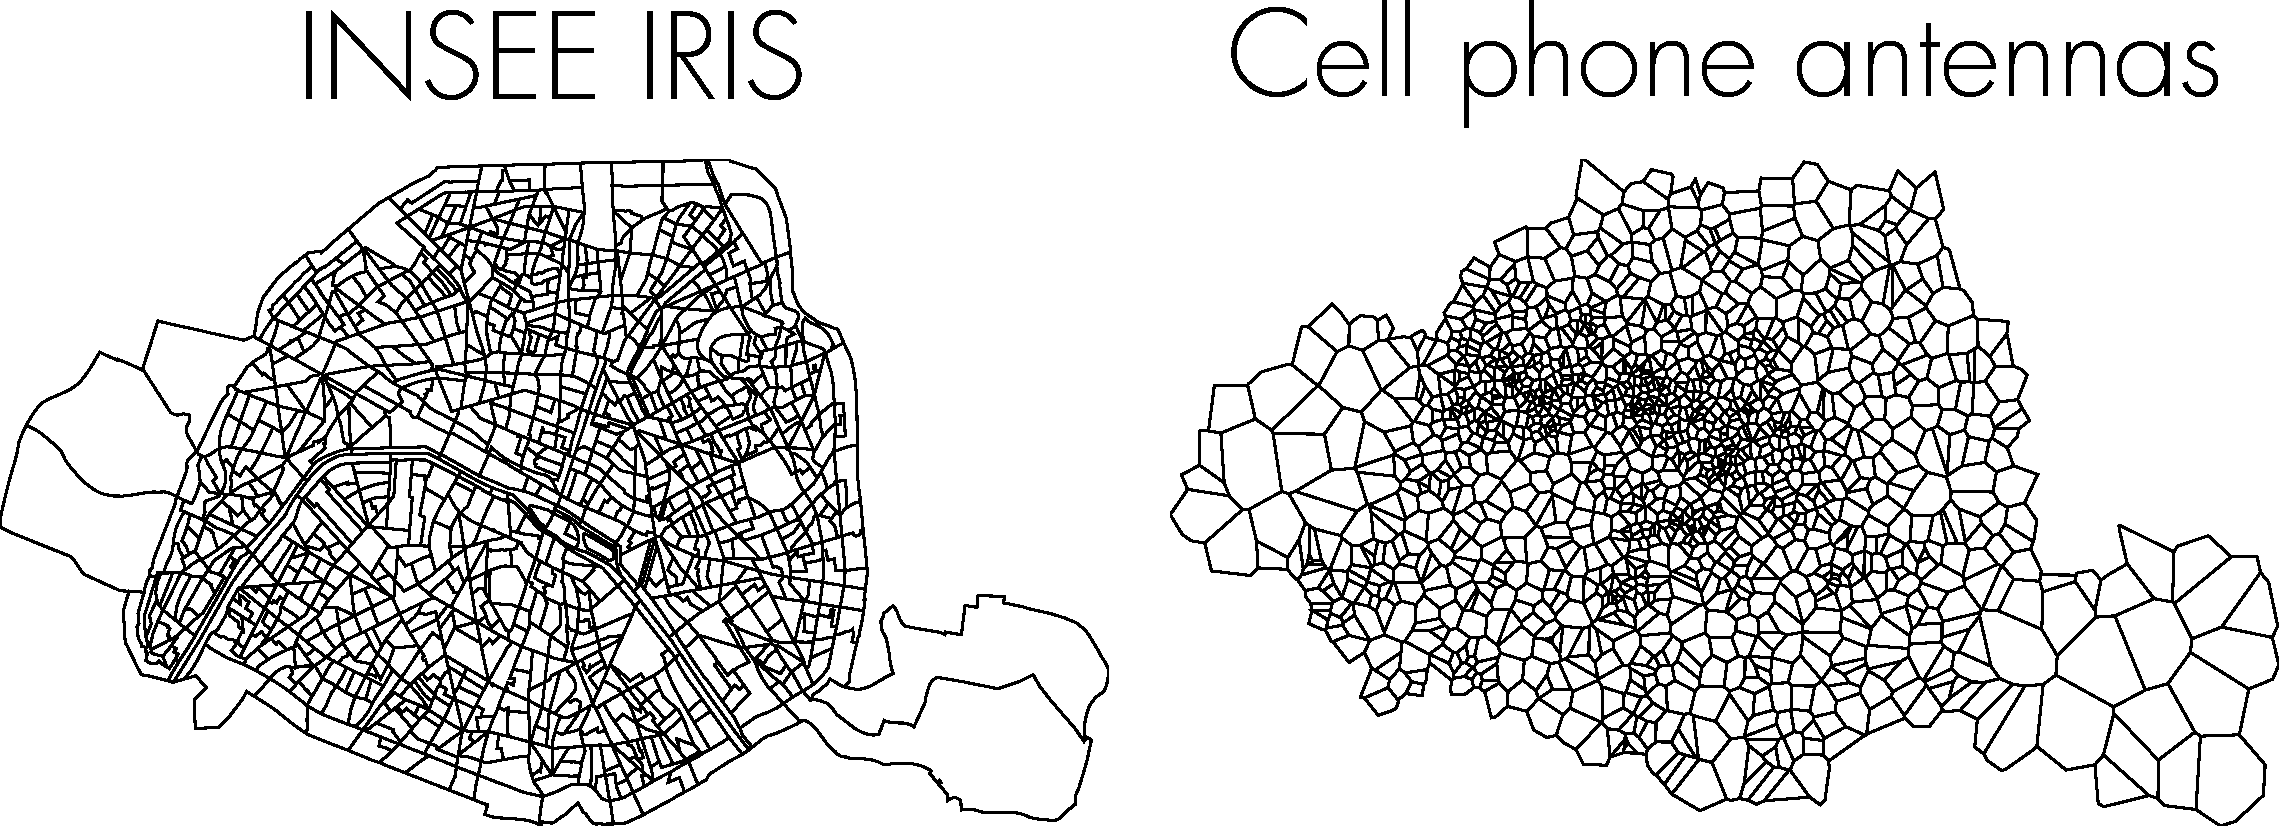
\includegraphics[width=\textwidth]{gfx/chapter-intro/IRIS_phone.pdf}
    \caption{(Left) IRIS zones in Paris, the smallest statistical units defined
    by the national statistics institute, INSEE. (Right) Voronoi tesselation
    built from the position of antennas of a popular french mobile phone carrier.
    There are $40\%$ more antennas than there are IRIS, and they tend to be more
    concentrated in zones of high daily activity (8th and 9th
    arrondissements).\label{fig:IRIS_phone}}
\end{figure}

Mobile phone data are spatially more precise. They give us a \emph{continuous}
information about the flow of individuals within the city, and not only
commuting.

But be careful. If they are ok to monitor aggregate
quantities~\cite{Lenormand:2014}, be careful of
individuals trajectories because sampled in a weird way.

    \subsection{A technological convergence}
    \label{sub:a_technological_convergence} 



Interdisciplinary collaborations already existed, data were already there. So
what is the qualitative difference between the state of the field say $20$ years
ago, and the state of the field as it is now, if any?\cite{Batty:2008,Batty:2012,Batty:2013} seeing the city as flows and networks.

\cite{Makse:1995} Modelling urban growth with diffusion limited aggregation
\cite{Rozenfeld:2008} Laws of population growth, using CCA algorithm to define
urban areas.


Agent-based models. Physicists have learned to be wary of the attempt to
describe in a deterministic framework the interactions of thousands, billions of
particles. Take a very simple model: the gas of hard spheres. Hard spheres are
simple objects: they have a fixed radius, cannot interpenetrate one another.
Their behaviour is well known, described by Newton's laws of motion, and we can
in theory solve all the equations describing their movements. In fact, we could
imagine, knowing the initial conditions, solve these equations and thus follow
the motion of every single particle (its position and speed) over time. In
practice, computers are way better than we are at doing that, and can easily follow for
us the trajectories of millions of spheres---I have coded that myself as a
student. So we have a very simple system, whose behaviour is perfectly known and
for which we can write exact dynamical equations, thus knowing perfectly its
time evolution at any arbitrary instant in the future. So what? What do we learn
from this simulated motion? What did we understand about the \emph{collective}
motion of spheres that we did not already know performing these simulations?
There is too much information for us to understand. In fact, there is as much
information in these simulations than there is in the original phenomenon, and
our understanding has not improved.
Facing the same questions, the fathers of statistical physics proposed to
extract some simpler, macroscopic information using probabilistic arguments.

Now, regarding social system, the context is even worse. We don't even know the
laws that determine the behaviour of individuals... we do not have the
equivalent of Newton's dynamics to describe the evolution of individuals in time
and their interactions. It is thus difficult what we would gain from simulating
the motions of thousands, millions of them using massive simulations. Even if
the laws were right, what would we learn from these simulations?

